\documentclass[11pt]{scrartcl}

\usepackage{cancel}
\usepackage[utf8]{inputenc}
\usepackage{mathtools}
\usepackage[sexy]{evan}

\title{11CSUR6}
\author{Himadri Mandal}

\begin{document}
\maketitle

\section{Solution}
\begin{soln}
	
\raggedright
I claim the answer is $(2n+1)(n+1)$.

\textbf{Construction} is simple enough: color the board with black stripes alternately.

To prove this we will induct.
Call the board $Q(n)$. Color $Q(n)$ as shown below, and call the \textbf{\color{yellow}\text{yellow}} part $Q(n-1)$ and the \textbf{\color{green}\text{green}} part $L(n-1)$.

\begin{center}
	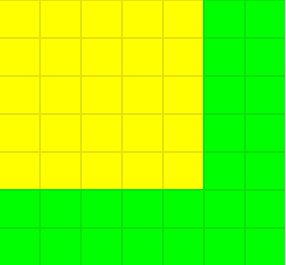
\includegraphics[scale=0.5]{../11CSUR6/11CSUR6.png}
\end{center}

Denote by $|Q(n)|, |L(n)|$ the maximum amount of black cells possible with the given coloring.

We know that $$|Q(n)| \leq |Q(n-1)| + |L(n-1)|$$.

\begin{claim}
	$|L(n-1)| = 4n+1$
\end{claim}
\begin{proof}
	This is actually pretty easy just induct.
\end{proof}

Now we will finish, assume $|Q(n-1)| = (2(n-1)+1)((n-1)+1)$ 
note that $$(2(n-1)+1)((n-1)+1)+(4n+1) = (2n+1)(n+1).$$ But that means $|Q(n)| \leq (2n+1)(n+1)$. 
So we are done.

\end{soln}
\end{document}
